\subsubsection{UC\theuccount-B - Redmine o GitLab inviano una segnalazione a Butterfly che la inoltra ad un utente Telegram o ad un indirizzo Email}
    \begin{figure}[H]
		\centering
		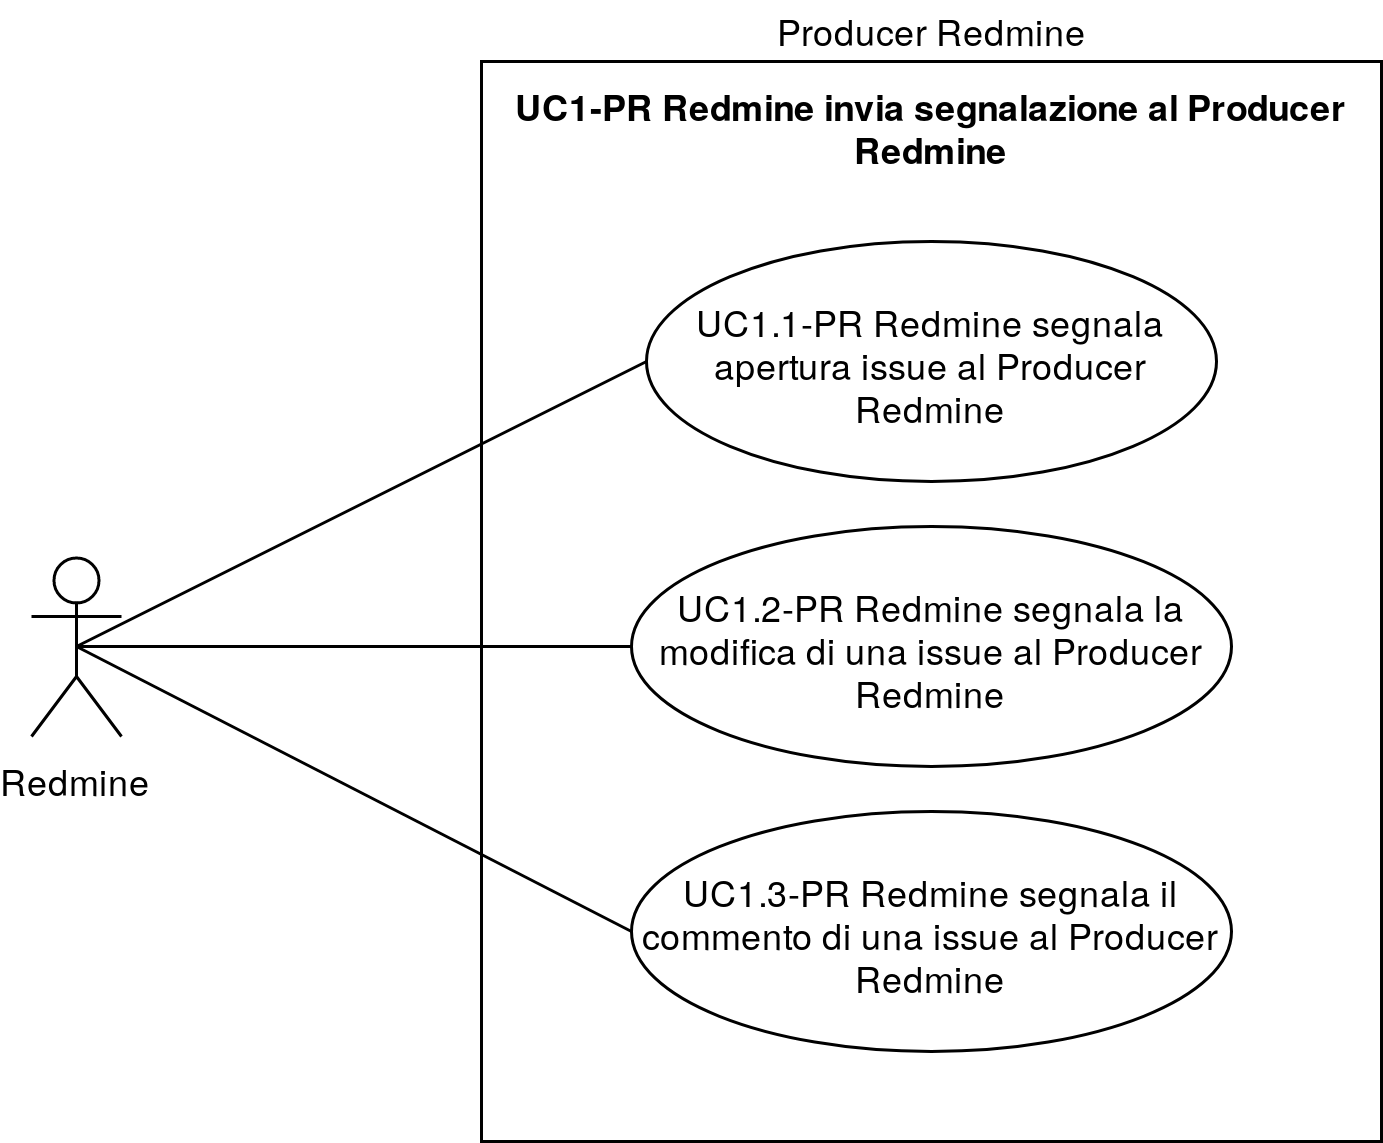
\includegraphics[width=0.7\textwidth]{img/casi_d'uso/UC1.png}\\
		\caption{UC\theuccount-B - Redmine o GitLab inviano una segnalazione a Butterfly che la inoltra ad un utente Telegram o ad un indirizzo Email}
	\end{figure}
	\begin{itemize}
		\item \textbf{Codice}: UC\theuccount-B.
		\item \textbf{Titolo}: Redmine o GitLab inviano una segnalazione a Butterfly che la inoltra ad un utente Telegram o ad un indirizzo Email.
		\item \textbf{Attori primari}: Redmine, GitLab.
		\item \textbf{Attori secondari}: Telegram, Email.
		\item \textbf{Descrizione}:  Redmine segnala a Butterfly l'apertura o la modifica di una issue di un particolare progetto. Lo stesso lo può fare GitLab segnalando l'apertura o modifica di una issue, con in più la segnalazione di un evento di push. In base alle impostazioni del Gestore Personale, tale segnalazione sarà inoltrata ad uno o più utenti Telegram o ad uno o più indirizzi Email.
		\item \textbf{Precondizione}: viene aperta o modificata una issue su Redmine, aperta o modificata una issue su GitLab, oppure viene effettuata un
		azione di push su GitLab.
		\item \textbf{Postcondizione}: l'utente Telegram o l'indirizzo Email selezionati ricevono la notifica delle segnalazione inviata da Redmine o GitLab.
		\item \textbf{Scenario principale}: 
		\begin{enumerate}
			\item Redmine o GitLab inviano una segnalazione al \progetto
			\item La segnalazione viene notificata attraverso Telegram o Email
		\end{enumerate}
		
	\end{itemize}